\chapter{Literature review}\label{chapter:relatedwork}
%Deterding et al. go on to explain that a gamified system, like a game, usually has rules and is goal oriented. Gamification is not a full-fledged game, although it utilizes many techniques that games implement such as, levels, clear goals, time constraints, badges, value conscious game design, challenge, limited resources and leader boards. It allows people to stay grounded in reality, whilestill profiting from successful game benefits like gaining access to a person’s emotions and intrinsic motivation, which in turn will help create habits. ZA ABRSTACT??
The following chapter provides an overview of the past research related to warm up (WU) as a preparatory exercise prior to performing physical activity, theories that describe and explain user's engagement and motivation when interacting with a gamified system and conceptually related works in the domain of gamified solutions relevant to fitness and exercise. In other words, this section explores the overlap of five different fields, namely exergames and gamification, health and fitness, injury prevention and motivational psychology. This concept is illustrated in Figure \ref{fig:diagram}.
\begin{figure}[h]
    \centering
    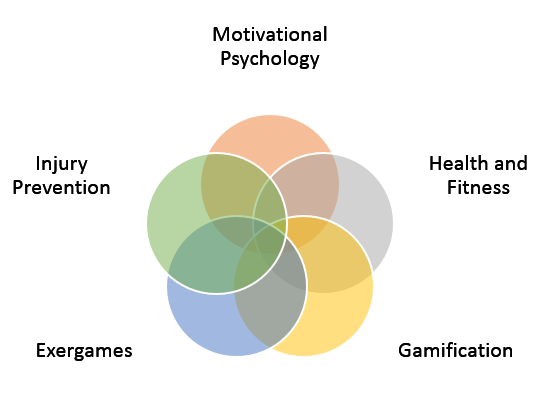
\includegraphics[width=0.75\textwidth]{diagram}
    \caption{The five general fields that relate to this work. The target field is presented as the overlap of the five fields}
    \label{fig:diagram}
\end{figure}
To impose structure, first the basic concepts related to WU and an overview of studies and results regarding the benefits of WU is given. Following, the concepts of gamification and exergames are introduced. Finally, a comparison between the presented approaches and our solution will be made together with the direction the
research in this thesis will take, and the motivations behind it.
\section{Warm Up in Sports}
\subsection{The Importance of Physical Activity}
In the last few decades, there has been a significant increase of women and men who engage in some sort of physical activity. Physical activity is beneficial to ones health. According to medical professionals, regular physical activity can significantly decrease the commonness of chronic diseases such as high blood pressure, heart disease,
(colon and breast) cancer, hypertension and diabetes as well as reduce cardiovascular-related deaths, to name a few \cite{mayr2015prevention, warburton2006health}. Regular exercise reduces the incidence of obesity
and obesity-related illnesses, maintains a general standard of health, and is associated with a reduced risk of premature death \cite{warburton2006health}. Moreover, regular engagement in sports of any kind can also pose as a countermeasure for psychological disorders and greatly limit the severity of
episodes of anxiety and depression \cite{mayr2015prevention}.
\subsection{Overview of Sports Injury}\label{subsection:injury}
The counterpart to all of the mentioned health benefits is that engaging in regular physical activity is often associated with a higher risk of injury which can occur in athletes of all age \cite{van1997severity}. To put it differently, there exists a higher risk of injury of the musculoskeletal system including soft tissue
damage, fractures, ligament and tendon tears, and nerve injuries in athletes who engage in some sort of physical (sport) activity \cite{mayr2015prevention}. Sport related injuries generally occur in joints: the knee, ankle, hip, shoulder, elbow, wrist and spine, usually from a sports related accident but often due to overuse, repetitive microtraumas that are solely insufficient to cause macroscopic injuries
 \cite{mayr2015prevention}. During international athletics championships between 2007 and 2014, data regarding injuries has been collected in order to compare the characteristics of injuries between female and male athletes \cite{edouard2015sex}. The results showed that males suffered more thigh strains than female athletes and that injury incidences differed between genders for location, type and event groups. The results concerning main injury locations for female and male athletes are presented in Figure \ref{fig:injuries}. The type of the injury depends on many factors, and usually is divided into: \textit{intrinsic} and \textit{extrinsic} \cite{mayr2015prevention}. The various types of injuries and their corresponding causes are presented in Appendix A. (TODO %\ref{chapter:warmup}
). Generally, extrinsic injuries are linked to the practice of sports itself and the environment the activity is catrried out. On the other hand, intrinsic injuries are tied to biological characteristics, anatomical factors, gender, and age, among others \cite{mayr2015prevention}. Other sports specialists group sport related injuries differently. For instance, Fischer \textit{et al.} (2016) differentiate between \textit{damage} as an overuse injury and \textit{injury} as an acute injury. They further state that an injury occurs in a single acute action (acute injury), while damage appears after repeated action as the result of many repetitive minor insults (overuse injury) \cite{fischer2016causes}. Addtitionally, in their book \textit{Overuse Injuries of the Musculoskeletal System}, Pecina and Bojanic (1993) state how ``the main characteristic of an injury is acuteness, whereas damage has a chronic character'' \cite{pecina1993overuse}. Acute injuries are more likely to occur in sports that include high-speed running, rapid movement, or full-body contact, whereas aerobic low-contact sports that include long training sessions may produce overuse injuries  \cite{mayr2015prevention}.
\begin{figure}[h]
    \centering
    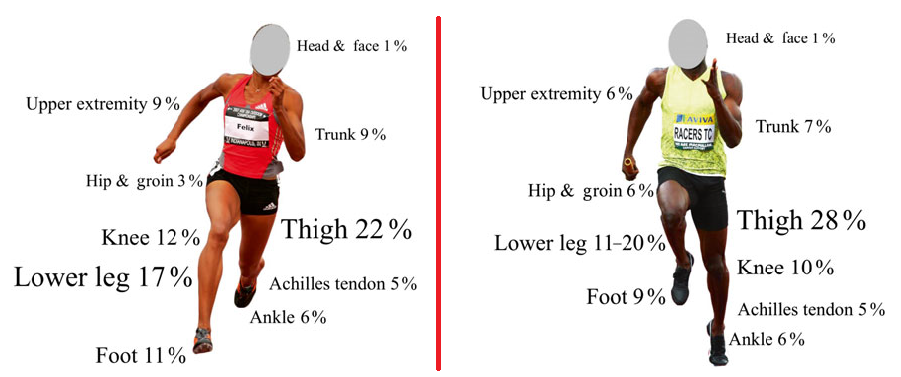
\includegraphics[width=0.85\textwidth]{injuries}
    \caption{Main injury location for female and male athletes during
international athletics championships from 2007 to 2014. Adapted from \cite{mayr2015prevention}}
    \label{fig:injuries}
\end{figure}\\
In order to prevent injuries, athletes should receive the correct amount of training and recovery period, and have a healthy lifestyle. The correct amount of training depends on the type of the physical activity itself, as much as the physical characteristics of the athlete. Moreover, the sports technique must be correct and, in case it is required, a good quality equipment should be used that is adapted to the player (morphology and level of play) in order to prevent injuries. Injury prevention strategies should be gender-specific. That is, as discussed in \cite{edouard2015sex} and presented in Figure \ref{fig:injuries}, for injury prevention ``one size does not fit all'', and hence it should be adapted to the differences in injury characteristics between female and male athletes. Lastly, as one of the main sports injury prevention mechanism, different studies outline that every physical activity must be preceded by a suitable WU procedure. This preparatory activity is hypothesized to give athletes sufficient time to adjust and prepare for a more intense susbsequent activity, and thus reduce the likelihood of injuries \cite{mayr2015prevention}.\\\\ Next, a definition and an overview of WU prior sports activities, together with its types and major benefits is presented.\pagebreak %NISI BAS PUNO O WARM UP + INJURY PREVENTION PISAO OVDE and should end with a cooling down phase . SVE ovo imas u onoj knjizi ove poslednje reference. mozda dodas nesto jos??  
\subsection{Defining Warm Up}
Despite very contrasting beliefs and limited scientific evidence regarding its effectiveness in many situations, WU has become a standard practice among professional and recreational athletes \cite{bishop2003warm1, bishop2003warm2, shellock1985warming}. WU in sports is defined as a period of preparatory exercise which is carried out in order to prepare the athlete for the demands of the subsequent physical activity  \cite{karvonen1992importance, woods2007warm, hedrick1992exercise}.
%karvonen skini i procitaj
Typically, WU includes a short and low-intensity preparatory activity which is followed by a stretching routine and sports specific exercise \cite{safran1989warm}. 
The ideal WU depends on the physical activity performed,
the level of competition, and the age of the participants. Moreover, the ideal WU should include the muscle groups that are required during the training or competition
 \cite{mayr2015prevention}. Various studies point out that the main purpose of WU is to enhance the subsequent competition or training performance and improve muscle dynamics to reduce the risk of sport-related injury \cite{bishop2003warm1, shellock1985warming, knudson2008warm}. 
 %HERE MENTION THE STUDIES THAT SAY THIS DOESNT HELP.  CHECK LEMON ILIEV
Nonetheless, there is still deficiency of scientific evidence on what kind of WU can influence both muscle damage prevention and performance improvement \cite{safran1989warm}.\\\\ The following section will shed lights on some of the assumed benefits of WU as a preparatory routine before physically more demanding exercise. 
\subsection{The Benefits of Warm Up}
Fradkin \textit{et al.} (2010) carried out a systematic review and meta-analysis of relevant studies concerning the benefits of WU on performance \cite{fradkin2006does}. They found that an adequate WU supports an improvement in performance in 79\% of the research studies analyzed. Furthermore, they pointed out that there exists little evidence supporting detrimental effects WU might have on performance and sports participants.
WU can affect the performance via variety of temperature and non-temperature related mechanisms \cite{bishop2003warm1}. 
%By performing a low intensity training routine before taking part in more demanding exercise, an increase in one's body temperature \(Magnusson 
%et al., 2000\) and muscle blood flow occurs \(Tiidus \& Shoemaker, 1995\).  
The most relevant effects of WU can be attributed to physiological mechanisms like increased muscle temperature, decreased resistance of muscle and joints (decreased stiffness), increased oxygen delivery to muscles, increased nerve-conduction rate and speeding of metabolic reactions \cite{bishop2003warm1}. 
However, the benefits of WU are not exclusively physical. Apart from the physiological changes a body undergoes during this preparatory period, it has been hypothesized that a possible psychological benefit can also be gained by following a proper WU routine \cite{bishop2003warm1,shellock1985warming}.
It has been suggested that WU can serve as a preparatory phase, providing time for athletes to concentrate and mentally prepare for the forthcoming exercise \cite{shellock1985warming}. 
%Thus, possible psychological benefits is increased mental preparedness for the forthcoming exercise\cite{bishop2003warm1}. 
Moreover, in the study that investigated the link between a WU and psychological processes, Ladvig (2013) reported that athletes who performed a proper WU routine before engaging in more demanding physical activity demonstrated significantly higher levels of exercise related motivation and enjoyment. Thus, increased motivation and enjoyment is an additional psychological benefit of WU \cite{ladwig2013psychological}.
 %findings of this theisis: http://aut.researchgateway.ac.nz/bitstream/handle/10292/325/WeerapongP.pdf?sequence=1
\\\\Apart from physiological and psychological benefits, WU has been suggested to have an important role in sports-related injury prevention \cite{shellock1985warming}. Unfortunately, there exist no high-quality research studies in order to draw a definite conclusion as to the effect WU has on sports-related injury prevention \cite{fields2007should}. Fradkin \textit{et al.} (2006) reviewed five high-quality studies that investigated the effects of warming up in humans on injury risk in physical activity \cite{fradkin2006does}. Five studies reported sufficient data on the effects of warming up on reducing injury risk in humans. However, only three of the studies found that performing a WU prior to performance significantly reduced the risk of injury in athletes, while the remaining two found that warming up has no effects in injury decrease \cite{fradkin2006does}. Therefore, the reearchers concluded that there is insufficient evidence to endorse or discontinue WU routine prior to physical activity in order to prevent injury among sports participants. However, the weight of evidence is in favour of a decreased risk of injury. Safran, \textit{et al.} (1989), proposed a possible bio-mechanical explanation for injury reduction with WU. The results of this study showed that warmed-up muscles in the animal models can elongate more before failure caused by increased force and length of stretch \cite{safran1989warm}.
%Furthermore, Nosaka and Clarckson found that high and low intensities of WU could reduce the magnitude musculatory damage ... They proposed that 
%A search of the literature identified only one published research paper on the effects of warm-up on the severity of muscle damage (Nosaka & Clarkson, 1997).  Nosaka and Clarkson (1997) found that both high (100 repetitions of maximal concentric contraction) and low (100 repetitions of minimal concentric contraction) intensities of 
%warm-up could reduce the magnitude of mu
%scle damage as indicated by reduced 
%soreness sensation, strength and range of 
%motion loss, swelling, and creatine kinase 
%activity.  The authors proposed that warm-up 
%might help to increase muscle temperature 
%and circulation, and consequen
%tly, increase muscle and conne
%ctive tissue el
%asticity
%the majority of effects of warm up have been attributed to temperature related mechanism
%TO DISCUSS STRETCHING! HERE %
%ne znam da li je ovo za komponenete dobro ovde? mozda bi trebao dodati jos nesto..
\subsection{The Types of Warm Up}
There exist various types of WU procedures that professional and recreational athletes at any level use as a preparatory phase before the physically more demanding exercise. According to \cite{safran1989warm}, an appropriate WU procedure should consist of three factors. These factors represent the WU components mentioned most often in the WU literature. However, recent studies question the importance and appropriateness of stretching as a component of a proper WU procedure [TODO]. The components are as follows:
\begin{itemize}
\item a period of aerobic exercise to increase body
temperature \cite{safran1989warm},
\item a period of sport-specific stretching to stretch 
the muscles to be used in the subsequent
performance \cite{safran1989warm}, and
\item a period of activity incorporating movements
similar to those to be used in the subsequent
performance \cite{safran1989warm}.
\end{itemize}  
First, it is important to distinguish between WU and stretching activities. While WU mainly focuses on core body temperature elevation, stretching involves movements that stretch the muscle in order to increase the range of motions of joints or group of joints \cite{knudson2008warm}. 
Generally, WU procedures can be classified into \textit{passive} and \textit{active} WU procedures, and are centered on increase in core and muscle temperature. However, they accomplish this objective through different approaches. The former involves raising muscle or core temperature by some external means (e.g. hot showers, saunas), while the latter aims to increase the body temperature through active movements of the major muscle groups (e.g. jogging, cycling, swimming) \cite{bishop2003warm2, shellock1985warming}. The most effective WU that could potentially affect the subsequent performance generally depends on the duration, intensity and the nature of the sports activity to be performed \cite{bishop2003warm2}. As each sport has its own unique requirements, it is difficult to specify a general WU routine that is beneficial and has a positive impact by maximizing the subsequent performance. Nonetheless, it is suggested that a proper WU should use general, whole-body movements and last 5-10 minutes, followed by a five minute recovery period \cite{bishop2003warm2}. However, in cold weather, the duration of the WU procedure should be increased \cite{mayr2015prevention}. %Vec si pisao o faktorima wu prethodno, pa ovde imas kontradikciju + You just mentioned performance, now introduce somehow injury prevention objasni zasto pises sad o injury prevention programu kad nema bas dokaza da ima efekta%
One example of WU procedure widely used in football which is easily adapted to other sports, is the \textit{FIFA 11+}, developed in cooperation with national and international experts under the leadership of the \textit{FIFA Medical and Research Centre }(\textit{F-MARC}), in order to reduce the incidence of football injuries and maximize the subsequent performance \cite{fifa}. The program includes various exercises that focus on core stabilization, and eccentric training of thigh muscles, to name a few. A recent review by Barengo \textit{et al.} (2014) showed how the FIFA 11+ program can decrease the incidence of injuries in amateur football players and also improve neuromuscular performance, enough to consider this program a fundamental public health intervention \cite{barengo2014impact}.\\*\\*
%reci da cemo koristiti vezbe koje su recommneded u fifa. dodaj za fatigue
%Several studies were conducted in the 1950s-1970s to investigate the effects of warming-up on athletic performance
%(Richards, 1968). In this context, approximately 60% of these studies found that warm-up was better
%to perform than no warm-up, whereas ~11% found that no warm-up was better, and the remaining ~29% found
%no significant differences between different protocols of warm-up and no warm-up (Blank, 1955). 
%tu sad das ove linkove
%(Generally, a warm-up to minimize impairments and enhance performance should be composed of a submaximal intensity aerobic activity followed by large amplitude dynamic stretching and then completed with sport-specific dynamic activities.
%these say that some stretching is ok
%http://www.jospt.org/doi/pdf/10.2519/jospt.1994.19.1.12
%https://www.ncbi.nlm.nih.gov/pubmed/21373870
%The efficacy, and characteristics, of warm-up and re-warm-up practices in soccer players: a systematic review. This review demonstrated that a static stretching WU reduced acute subsequent performance, while WU activities that include dynamic stretching, PAP-based exercises, and the FIFA 11+ can elicit positive effects in soccer players. The efficacy of an active RWU during half-time is also justified.
%ovo se placa nesto 
 %http://greatist.com/fitness/stretching-dynamic-warmup-040413
Although considering the aforementioned benefits and the fact it is widely recommended to undertake the practice of WU, many amateur and recreational athletes do not seem to perform a proper WU before an exercise \cite{fradkin2010effects}. The reasons for this are manifold. Some people do not realize the importance of WU, find it tiresome or being pressed for time and eager for instantaneous results, start with the more strenuous activity immediately. A recent survey carried out by Fradkin, \textit{et al.} (2010)  which included 1040 golfers and their WU habits, revealed the most common reasons for not warming-up \cite{fradkin2010effects}. The survey showed that out of all the questioned golfers, over 70\% never or rarely warm-up. The most common reasons for not performing a proper WU routine were the perception that WU is needless (38.7\%), lack of time (36.4\%) and that they do not want to be bothered with this routine (33.7\%).
% A survey of 1040 randomly selected golfers was conducted over a 3-week period in July 1999. Information about golf participation, usual warm-up habits and reasons for these warm-up behaviours was obtained by a verbally administered self-report survey. Over 70% of the surveyed golfers stated that they never or seldom warm-up, with only 3.8% reporting warming-up on every occasion. The most common reasons why golfers warmed-up included to play better (74.5%), to prevent injury (27.0%), and because everyone else does (13.2%). Common reasons for not warming-up were the perception that they don't need to (38.7%), don't have enough time (36.4%) and can't be bothered (33.7%).
These results suggest that educational and motivational solutions with primary focus on the benefits of WU, including injury prevention, need to be developed and implemented in order to increase the proportion of athletes who engage in WU routines before every strenuous exercise. One possible solution is the usage of \textit{Gamification} and \textit{Exergames} in motivating athletes to perform WU more regularly. 
\pagebreak
\section{Gamification and Exergames}
Having outlined the basic concepts of WU procedures, the following section sheds light on the dimensions of Gamification and Exergames. In order to tie in with the idea of linking these concepts with WU procedures, the emphasis will be placed on understanding the fundamental aspects behind human's motivation (Section   \ref{chapter:motivation}). Subsequently, we dive deep into techniques, elements and benefits of Gamification and Exergames.
\subsection{Video Games and Exercise}
At first glance, most people think of video games and exercise as two concepts that are polar opposites and cannot coexist together. Exercise and sports are usually tied to being physically active and burning calories. On the other hand, video games are usually linked to activities that involve hours of sitting down by your self to play \textit{World of Warcraft}\footnote{Or even \textit{Flappy Birds}}. However, these two concepts are actually made to go alongside another. In both instances, one is seeking to be better at the task being performed. For example, an athlete will try to improve its best running time, and the video gamer will strive to beat its best game score. The missing link, that connects these activities together, is given in a form of \textit{Gamification} which leverages people's natural desires for competition, socializing, learning, mastery, achievement, status, self-expression, and closure in order to encourage and motivate individuals to exercise more frequently and improve their overall health.
%http://link.springer.com/chapter/10.1007%2F978-3-319-07127-5_23
%(http://www.enterprise-gamification.com/mediawiki/index.php?title=Category:Gamification_Design_Elements)
% are commonly used 
%check this here https://badgeville.com/wiki/health
%% add gamification example reference
% http://www.enterprise-gamification.com/mediawiki/index.php?title=Gamification_Examples
\paragraph{A Primer on Gamification}
In recent years, there has been a tremendous increase in popularity of video games inspired software solutions designed to address issues in a variety of functional areas, incentivize consumer behavior or increase motivation and the desire for achievement. What these software solutions all have in common is that they are based on the concept of \textit{Gamification}. This term has begun to rise in popularity in 2010 (Figure \ref{fig:buzz}), and since then has been a trending topic. %ovde dodaj 
%It has proved to be an effective tool for certain businesses for developing new skills, solve problems, improve results or address.
Gamification is being used and studied in various domains, from education and academic performance to health care, finance, company culture building and recruitment, to name a few \cite{gamificationExamples, gamificationWiki, enterpriseGamify}. Large companies like \textit{Nike} \cite{nikePlus}, \textit{Deloitte} \cite{deloitte}, \textit{Starbucks} \cite{starbucks}, \textit{Coca Cola} \cite{coke}, and \textit{Toyota} \cite{toyota} have all used gamified solutions in order to increase customer loyalty, change behaviors, and drive innovation. \pagebreak 
\begin{figure}[h]
    \centering
    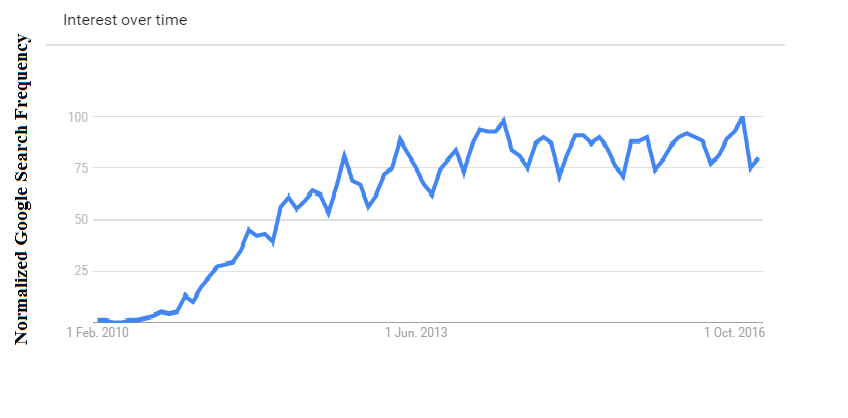
\includegraphics[width=\textwidth]{buzz}
    \caption{Google search frequency of the term \textit{gamification} from Janauary 2010 through January 2017. Data source: Google Trends, www.google.com/trends}
    \label{fig:buzz}
\end{figure}\\
Gamified solutions for sports activities are becoming popular and widely used also, and according to \cite{iosPopulatity} the consumer segment comprised of \textit{Millennials}, have the highest inclination towards iOS fitness mobile applications (Figure \ref{fig:iosApps}). 
\begin{figure}[h]
    \centering
    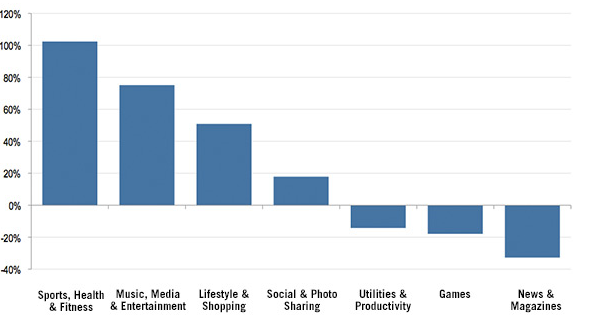
\includegraphics[width=0.85\textwidth]{iosApps}
    \caption{Addopted from \cite{iosPopulatity}: Random sample of 15271 American iOS owners}
    \label{fig:iosApps}
\end{figure}\\
An example is the \textit{Strava} application and website that uses gamification elements in order to enhance the experience of sport and connect athletes with similar sports affinities from around the world \cite{strava}. %samo dodaj linkove za kompanije websajte
Moreover, there is an increasing number of startups (e.g. \textit{Foursquare}, \textit{CodeAcademy}) that have gamification  at  their  core \cite{codeacademy} or offer assistance to enterprises to gamify their existing services (e.g. \textit{Badgeville} \cite{badgeville}). Hamari \textit{et al.} (2014) reported on an increasing popularity of gamification related researches in the academia \cite{hamari2014does}. Figure \ref{fig:pub} gives an overview of the increase of writing on this topic. The figure includes only the number of publications for every year for the term \textit{Gamification} and excludes patents and citations. 
\begin{figure}[h]
    \centering
    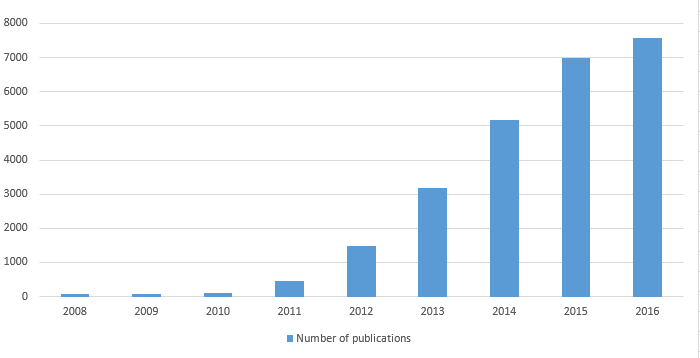
\includegraphics[width=\textwidth]{pub}
    \caption{Search hits on 'Gamification'. Data source: www.scholar.google.com}
    \label{fig:pub}
\end{figure}\\
It is worth noticing that the appearance of the term Gamification titles of publication has been increasing more rapidly than search hits for the same term (see Figure \ref{fig:buzz}). This suggests that Gamification is becoming more popular in academic circles as a research topic.TODO%read fred's comments on this + change years 
\paragraph{A Primer on Exergames}
Recent progressions in ubiquitous technologies offer a solution that could dispute a number of potential barriers preventing individuals to engage in regular physical activities. This solution comes in a form of video games that are developed for a certain purpose other than entertainment alone, mainly for the context of health and fitness, named \textit{exergames}. They represent enjoyable tools that can increase the energy expenditure during game play, motivate players to engage in physical activity more regularly, promote social interaction, and even enhance cognitive performance \cite{staiano2011exergames}. Compared to the term gamification, the term exergame or \textit{exergaming} has been known for a while, and its roots can be found in games released in the late eighties. The name exergame is a concatenation of the words \textit{exercise} and \textit{game}, sometimes referred to as \textit{Active Video Gaming} (AVGs) \cite{altamimi2012survey}. This genre includes video games with the aim of encouraging and facilitating physical activity which rely on technology that tracks body movement or reaction \cite{altamimi2012survey}. A large amount of research has been put into exergames development, and there exist several successful commercial
products today. The \textit{Nintendo Wii} \cite{wii}, released in November 2006 for the home entertainment market, was the first mainstream game console which contained a built in exergaming system. Nintendo Wii exergame contributed to a 73\% increase in Nintendo's net sales, with 24.5 million consoles and 148.4 million software units sold to date, making it the second highest selling video game in 2007 \cite{staiano2011exergames}. Apart from exercise, exergames have been used in fields such as art, education, and rehabilitation  \cite{altamimi2012survey}. Researches found the the usage of exergames in these fields has led to the 
development of educational and social skills \cite{altamimi2012survey}. Moreover, one important skill that exergames can build on is children's motor skills \cite{delgado2009low}. Taking into account all the mentioned benefits one can gain with exergames, it is understandable that there is also an increase of writing on this topic (Figure \ref{fig:pubEx}). As in the former figure on gamification, this one also includes only the number of publications for every year for the terms \textit{exergame} or \textit{exergaming} and excludes patents and citations. 
\begin{figure}[h]
    \centering
    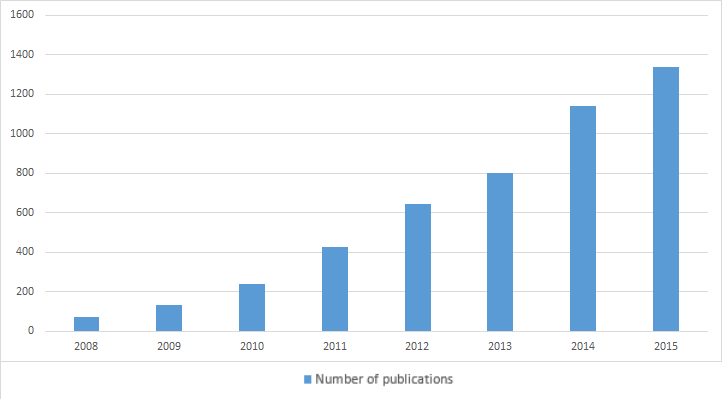
\includegraphics[width=0.9\textwidth]{pubEx}
    \caption{Search hits on 'exergame' or 'exergaming'. Data source: www.scholar.google.com}
    \label{fig:pubEx}
\end{figure}\\
Exergames do an excellent job of implementing various gamification techniques that play off person's desire to master certain skills or achieve a specific goal. By breaking down the barriers to traditional exercise and workouts, they have the potential to promote physical activity and stimulate behavioral change, within a fun, enjoyable and motivating context. Researchers agree how incorporating exergames into schools, fitness centers, and homes can promote healthy youth development and even combat the childhood obesity crisis \cite{staiano2011exergames}. \\
The player forms the root of Gamification and, in any system, the outcome is affected and driven by his motivation \cite{zichermann2011gamification}. Therefore, to understand the potentials and fundamental aspects behind Gamification and Exergame, one important part is to understand what drives people's motivation. Thus, in  order  to  create  an  effective  gamified system, one needs to understand  how  human  nature  works  and  how  it can be influenced and shaped. For this reason, the next sections introduce different views from psychology about motivation and explain what has to be considered in terms of truly engaging individuals, and how Gamification can use this in order to achieve its purpose. 
\pagebreak
\section{Theories of Motivation}
\label{chapter:motivation}
There are two main purposes of this section. The first is to provide a suitable overview of the subject itself and to introduce terms that will be used later in the discussion. The second purpose is to present theories that describe and explain various psychological effects that games have on players and how can they be used to enhance user's engagement and motivation when interacting with a gamified system. Two important theories that are regarded as important foundations for  the  concept of Gamification are presented. First, the \textit{Self Determination theory} introduced by Ryan and Deci, and then the \textit{State of Flow} by Mihaly Csikszentmihalyi are discussed. 
\subsection{The Rules of Motivation}
The main purpose of gamification is to ``\textit{help people get from point A to point B in their lives}'', whether it is visiting the gamified system more often, learning a new language, or exercising more \cite{gamificationPurpose}. Gamification is about stimulating
 individuals to act in a certain way, or at least to develop an inclination for certain behavior. The root of gamification is human motivation.\\\\The word \textit{motivation} originates from Latin \textit{motivus} and stands for ``\textit{serve to move}''. In other words, motivation can be interpreted as ``\textit{to be moved to do something}''\cite{ryan2000intrinsic}. It can be defined as ``\textit{those forces within an individual that push or propel him to satisfy basic needs or wants}'' \cite{pardee1990motivation}. One of the most influential researchers in the domain of human motivation and behavior, Richard M. Ryan and Edward L. Deci, argue that people \textit{can be moved} to act by various types of factors, as so with highly diverse experiences and consequences \cite{ryan2000intrinsic}. For example, people can be motivated because they value the activity they perform, or because there exists some external influence and pressure. Furthermore, they point out that each person has different amounts and also different types of motivation. That is, each person is different in level (i.e. amount) and orientation (i.e. type) of their motivation, whereas orientation might be a goal which gives rise to action and therefore governs human behavior. Gamification taps exactly in these forces within an individuals that push or propel them to satisfy certain needs or wants. It exposes complex, but learnable systems that individuals can engage with to achieve personal mastery and, hence, meet their objective \cite{gamificationPurpose}.\\\\
There exist various motivation theories that address different aspects of motivational properties of gamified systems. However, only two theories are further discussed in details because they have already been applied to great number of digital systems which makes them an understandable starting point in understanding gamification and its influence on players' motivation. \pagebreak

\subsection{Self Determination Theory}
%deci ima dva papera
One of the most influential motivational theories is the \textit{Self Determination Theory} (SDT) introduced by Ryan and Deci \cite{deci1994promoting, ryan2000self,ryan2000intrinsic, deci2000and}. It is an empirically derived theory of human motivation that makes distinctions between different types of motivation in terms of reasons and goals that cause the respective action. That is, SDT proposes that behaviors that are intentional might vary in the extent to which they are \textit{self-determined} versus \textit{controlled}. This means that behaviors can vary in the extent they are experienced as being freely chosen and coming from one's self in contrary to being pressured or controlled externally. When these behaviors are experienced as freely chosen they are considered self-determined or autonomous, whereas the extent they are experienced as coerced, they are considered controlled \cite{deci1994promoting}. Having this in mind, SDT distinguishes between \textit{intrinsic} and \textit{extrinsic} motivation \cite{ryan2000intrinsic}. The first type of motivation, as the word \textit{intrinsic} already suggests, refers to performing an activity for the inherent satisfaction. When intrinsically motivated, a person is moved to act because the activity is challenging, interesting and enjoyable on its own rather than because of some external prods, pressures, or rewards. On the other hand, extrinsic motivation refers to performing an action because it leads to \textit{separable outcome}. That is, there is some external reward or influence which drives the person to accomplish the task. The comparison between people intrinsically and those extrinsically motivated reveals that the former have more interest, excitement, and confidence which in turn, can not only enhance performance, persistence, and creativity but consequently boost vitality, increase self-esteem and general well-being \cite{ryan2000self}. Though this division is for most people intuitively understandable, it is not always as clear as it may seem. For example, as the SDT theory states, ``\textit{motivations are fluid}''. Hence, people can convert extrinsic motivators to intrinsic if they internalize the desire to do so. To put it more simply, in a situation where the extrinsic motivator is found meaningful, pleasurable and consistent with a person's worldview, it can be perceived and adopted as if it was intrinsic \cite{zichermann2012}.
Although, in one sense, intrinsic motivation can exist within an individual, in another sense, it can exist in the relation between the individual and the activity one performs. Having that in mind, it is important to point out that not everyone is intrinsically motivated for the same activities and that not everyone is intrinsically motivated for any particular activity \cite{ryan2000intrinsic}. \\In SDT, the \textit{basic psychological need satisfaction} is assumed to be the core motivational mechanism that directs human's behavior. SDT postulates three innate psychological needs (Figure \ref{fig:ss}), that are ``essential for ongoing psychological growth, integrity, and well-being'' and all three of them play a necessary part in optimal development, hence none can be disregarded without significant negative consequences. These needs are the need for \textit{autonomy}, \textit{competence} and \textit{relatedness}. When individuals experience them, they become self-determined and intrinsically motivated to pursue things that interest them the most \cite{deci2000and}.\\\\\\ %https://selfdeterminationtheory.org/SDT/documents/2010_VandenBroeckVansteenkisteNSscale_JOOP.pdf
The basic psychological needs as defined by Ryan and Deci are as follows:
\begin{itemize}
\item \textbf{Autonomy} represents individuals' innate desire to feel ``\textit{free}'', to experience a sense of choice and psychological freedom when carrying out certain activities \cite{deci2000and}. Situations in which individuals are provided with the opportunity to choose freely, accompanied with a positive feedback, have been shown to influence and improve autonomy and, hence, the intrinsic motivation of individuals \cite{ryan2000self}. For example, students are  autonomous when they willingly spend time and energy for completing their assignments. 
\item \textbf{Competence} represents individuals' innate desire to feel ``\textit{effective}'' when interacting with the environment. For example, students are competent in cases when they feel they can meet the challenges of their schoolwork. Furthermore, Ryan and Deci point out that positive feedback can signify effectance and provide a satisfaction of the need for competence and consequently enhance intrinsic motivation. Contrarily, negative feedback that convey ineffectance, tend to diminish the sense of competence and hence undermine individuals' intrinsic motivation. 
%A. P. Hill, "A Brief Guide to Self-Determination Theory," September 2011. [Online]. Available: http://www.heacademy.ac.uk/assets/hlst/documents/projects/round_11/r11_hill_guide.pdf. [Accessed 10 April 2013].
\item \textbf{Relatedness} corresponds to experiencing meaningful ``\textit{connection}'' to others. To put it differently, relatedness corresponds to ones innate need to to be a member of a group, to love and care, and to be loved and cared for \cite{broeck2010capturing}. This psychological need is satisfied when individuals experience a sense of togetherness and develop a close and intimate relationship with others.\\
\end{itemize}
\begin{figure}[h]
    \centering
    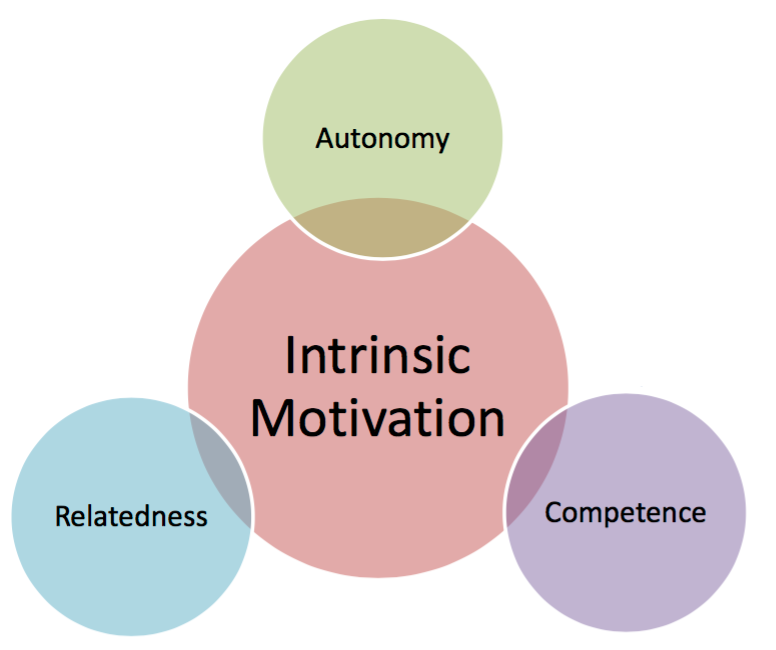
\includegraphics[width=0.6\textwidth]{ss}
    \caption{Basic psychological needs according to Ryan, R.M. \& Deci E.L. \cite{deci1994promoting} }
    \label{fig:ss}
\end{figure}
The specification of autonomy, competence, and relatedness is important because it allows the prediction of variables that can affect individual's intrinsic motivation and the development of their extrinsic motivation \cite{deci1994promoting}. Gamification and exergames achieve these needs by means of diverse game elements, which will be discussed in detail in the subsequent sections.\\\\
Despite the observable evidence that humans, in general, can have intrinsic motivational tendencies towards some activities, this bias appears to manifest only in certain conditions and circumstances. Hence, SDT also places much emphasis on understanding conditions that enhance and sustain versus subdue and diminish intrinsic motivation \cite{ryan2000intrinsic}. A sub-theory of SDT called \textit{Cognitive Evaluation Theory} (CET) was presented by Deci and Ryan in 1985, and focuses on social and environmental factors that promote or undermine this type of motivation. It uses language that reflects the assumption that intrinsic motivation, is rather catalyzed than caused when individuals are in appropriate socio-enviromental circumstances \cite{ryan2000self, ryan2000intrinsic}. In other words, intrinsic motivation does not occur by itself, but represents the outcome of one's interaction with the environment and one's interests and preferences. That is, intrinsic motivation ``\textit{will flourish if circumstances permit}'' \cite{ryan2000self}. Furthermore, CET, which focuses mainly on the fundamental needs for competence and autonomy, argues that interpersonal events and structures, such as rewards, communication or feedback can increase intrinsic motivation for certain actions because they satisfy the basic psychological need for competence. Accordingly, it is predicted that optimal challenges, positive feedback and freedom from degrading evaluations promote intrinsic motivation, while tangible rewards, threats, deadlines  and  directives decrease it \cite{ryan2000self}. CET also argues that the satisfaction of the psychological need for competence will not enhance intrinsic motivation unless it is joined by a sense of autonomy. Hence, people must perceive that their behavior is self-determined in order for intrinsic motivation to be maintained or enhanced. In other words, for a high level of intrinsic motivation, the needs for competence and autonomy must both be satisfied \cite{ryan2000self}. It is important to point out, as stated by Ryan and Deci, that people will be intrinsically motivated for certain activities only when they are intrinsically captivating for an individual. This includes activities that offer a degree of novelty, challenge or aesthetic value. Activities that do not provide such appeal, will not be experienced as intrinsically motivated. \\\\
Even though intrinsic motivation is of great importance, most of the activities people engage in are not intrinsically motivated. Such activities, being uninteresting and unsatisfactory for individuals  require external \textit{push} in order to be realized. This motivation, contrary to intrinsic motivation which refers to doing an activity simply for the enjoyment of the activity itself, is known as extrinsic motivation. It refers to performing certain activities because it is expected to result in some additional outcome or reward that have an instrumental value for the individual performing that action \cite{ryan2000self}. In general, extrinsically motivated behaviors are ones that would not happen instinctively, and hence must be prompted by an intrumentality \cite{deci1994promoting}. Various studies demonstrated that in specific circumstances extrinsic motivation can sustain intrinsic motivation, thus suggesting that extrinsically motivated behaviors can also be self-determined \cite{deci1994promoting}. Extrinsically motivated behaviors become self-determined through the process of \textit{internalization} and \textit{integration}. Internalization involves transforming internal regulatory processes into internal regulatory processes, while integration corresponds to the process of integrating these now internalized values and regulation into one's self \cite{deci1994promoting}. There exist four types of extrinsic regulation that can result from different types of internalization and integration, which were introduced within SDT as a subtheory called \textit{Organismic Integration Theory} (OIT) \cite{ryan2000intrinsic, ryan2000self, deci1994promoting}. For instance, students who work on their assignments because they personally understand its importance for their future career and those who do it only to adhere to their parents' control are both extrinsically motivated. Even though both cases involve instrumentalities rather than enjoyment, the former entails personal endorsement and a feeling of choice while the latter is associated only with an external regulation.\\
Figure \ref{fig:tax} illustrates the IOT taxonomy of motivational types arranged from left to right in terms of the degree to which the motivation originates from the self (i.e. are self-determined).\\ 
\begin{figure}[h]
    \centering
    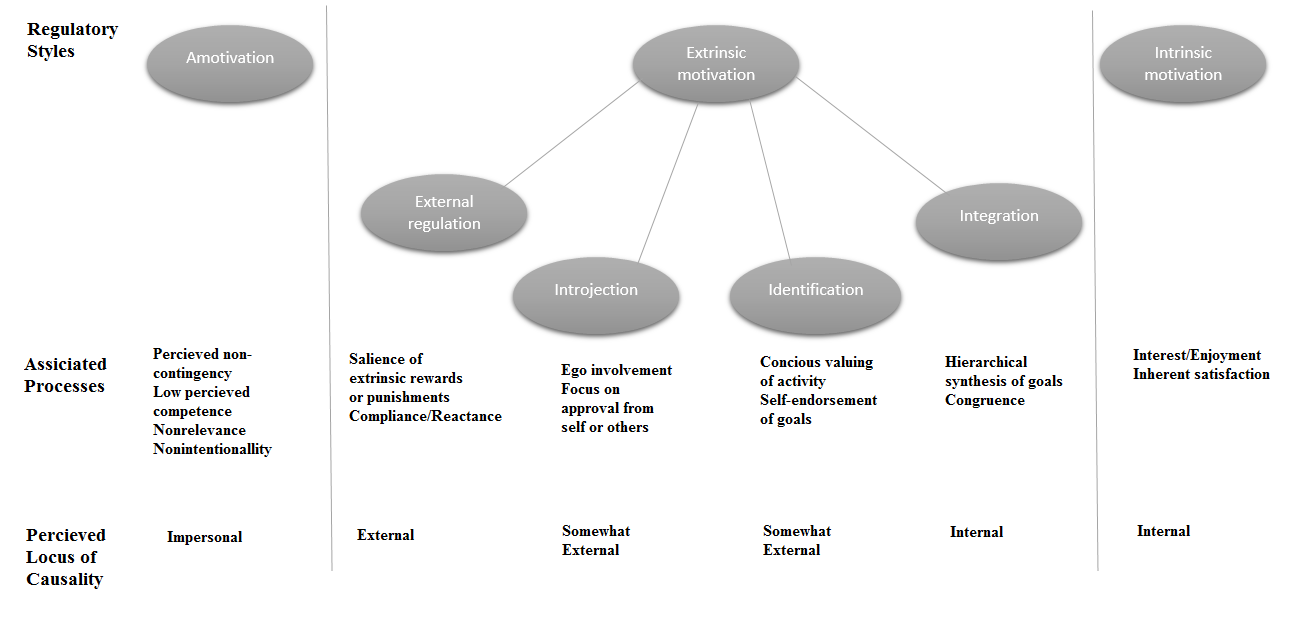
\includegraphics[width=\textwidth]{taxm}
    \caption{Based on Ryan, R.M. \& Deci E.L. Self-Determination Continuum showing types of Motivation}
    \label{fig:tax}
\end{figure}\\
First, the extrinsically motivated behavior that is the least autonomous is known as \textit{external regulation} and is regulated through some external means, such as rewards and constraints. For example, an athlete who participates in the Olympics only to obtain a medal represents an instance of externally regulated behavior. In case of \textit{introjected regulation}, individuals begin to internalize the reasons for their action. However, this internalization only replaces the external source of motivation with an internal one, such as guilt, worry or shame. That is, when people are motivated to perform activity in order to maintain feeling of worth. An example for introjection is the athlete who goes to the practice just because he would feel guilty if it has been skipped. A more autonomous type of extrinsic motivation, \textit{identification}, manifests when a person identifies with the importance of some behavior and accepts it as a personal regulation only because it benefits the athlete in achieving a specific goal. An example for this behavior is a runner who does not like weight lifting, but nevertheless chooses to to do it because it will positively impact her future performance. \textit{Integrated regulation}, as the most autonomous of extrinsic motivation that shares many qualities with intrinsic motivation, is a form of motivation that arises when an individual has fully assimilated the identified regulation within himself. An example of integrated regulation is an athlete who chooses to postpone the night out with his friend in order to be in good shape for the next day's tournament. Integration together with intrinsic motivation represent the core for self-determined functioning and they both share the qualities that constitute self-determination. Even though they might seem quite similar, they are different in the sense that intrinsically motivated behaviors are ``\textit{autotelic in nature}'' while, on the other hand, integrated behaviors are ``\textit{instrumentally (though freely) performed}'' for the outcome that is self satisfactory.  Finally, the self-determination continuum is closed with  \textit{amotivation} which represents ``\textit{non-regulation}'' from the SDT perspective as it refers to a state where intentions to act are non existent. A person amotivated towards exercise would not exercise at all, 
or engage in exercise in a passive and disorganised  manner \cite{vallerand2007intrinsic, ryan2000intrinsic, deci1994promoting}.\\\\
Having outlined the basic concepts behind SDT, the next section covers the link between them and gamification. That is, we further detail how gamification makes advantage of the foundations of SDT.
\subsubsection{Gamification and SDT}
In their book \textit{For the win. How Game Thinking can revolutionize your business} (2012 )\cite{werbach2012win} Werbach and Hunter state that ``games are perfect illustration of the lessons of SDT''. They point out how even simple games activate intrinsic needs for autonomy (because it is up to the player how to solve a challenge), competence (sense of accomplishment if certain goal is achieved) and, lastly, relatedness (when the the achieved results are shared among group of friends). The same way as games, Gamification uses these three innate motivators in order to generate results.
What are the specific takeaways for a successful gamification?
- Rewards can crowd out fun
- Boring can be engaging
- Tune your feedback
Tangible and expected extrinsic rewards can damage intrinsic motivation and interesting tasks (Werbach and Hunter,2012, p.60). On the other hand, extrinsic rewards can also have a positive effect when people need to accomplish boring
tasks (Werbach and Hunter,2012, p.62).
NOT COMPLETED-TODO:add relation to the warm up scenario? how do we plan to address autonomy, relatedness and competence? 
\\*

\subsection{State of Flow}
TODO: is the state of flow realistically achievable in 15 minutes or short intervals? to argue. so you need to look into how much time is needed to reach this state?

Mih\'{a}ly Cs\'{i}kszentmih\'{a}lyi, one of the most recognized game psychologists and a professor at University of Chicago, described in 1975 for the first time the phenomenon of \textit{flow}. Being fascinated by artists who would essentially get lost in their work Cs\'{i}kszentmih\'{a}lyi argued how, creative people might differ from one another in many ways but they always have one thing in common. They love what they do. Their love for a particular activity is not because of a potential outcome or a reward. What drives them is solely the opportunity to do what they enjoy doing \cite{csikszentmihalyi1996flow}. Athletes often refer to this concept as ``being in the zone,'' religious mystics
as being in ``ecstasy,'' artists and musicians as ``aesthetic rapture'' \cite{csikszentmihalyi1997finding}. In order to explain this experience, Cs\'{i}kszentmih\'{a}lyi has interviewed individuals willing to devote many hours to their avocations without asking for external rewards. After a series of studies, based on the individuals' responses regarding their emotions while performing certain activity they enjoy, Cs\'{i}kszentmih\'{a}lyi  developed a theory of optimal experience based on the concept of \textit{flow}, which he describes as 
``the state in which people are so involved in an activity that nothing else seems to matter; the experience itself is so enjoyable that people will do it even at greater cost, for the sheer sake of doing it'' \cite{flow1990psychology}. Flow is also considered as an optimal state of intrinsic motivation, where people become absolutely immersed in what they are doing, they forget about physical feelings, passage of time, and their ego fades away \cite{lithiumGamification}. 
It represents a state in which one feels in control, fully immersed and motivated, at the top of its abilities and neither overwhelmed by difficulty nor uninterested. Cs\'{i}kszentmih\'{a}lyi \textit{et. al} (2004) state the flow experiences are relatively rare in everyday life, however, various activities are able to produce them, provided certain conditions are met. They further argue that three conditions have to be met in order to achieve a flow state. First, a state of flow needs clearly defined set of goals which must guide the user and give purpose to the behavior \cite{csikszentmihalyi2014flow}. However, sometimes the goals of some activities cannot be perfectly clear for the individual, as in the case of creative activities. Nonetheless, it is possible for a person to develop a strong personal sense of what is intended to be done by performing the activity \cite{kiili2006evaluations}. The second condition for obtaining the state of flow is the presence  of clear and immediate feedback. It informs the user if he/she is succeeding in a specific goal and how to adjust his or her performance according to the ``continually  changing environment demands'' \cite{csikszentmihalyi2014flow}. Lastly, one of the most important condition is to maintain balance between perceived challenges and perceived skills \cite{csikszentmihalyi2014flow}. When experiencing a flow, a person's skill is at just the right level to cope with the situational demands.\\*
Nakamura and Cs\'{i}kszentmih\'{a}lyi (2012) further argue that under these three conditions, individuals can enter a state with the following characteristics:
\begin{itemize}
\item Control. A sense that one has skills sufficient enough to minimize the margin of error to close to zero and, therefore, can in principle deal with and fully enjoy the current situation because one knows how to respond to any anything that can happen next \cite{csikszentmihalyi2014flow}. Moreover, this sense of control is believed to be one of the important flow antecedents in games\cite{kiili2006evaluations}. 
\item Action–awareness merging. The flow state is so involving that, during it, it affects the individual in a way that the activity performed becomes spontaneous and automatic.
\item Concentration. While in flow, one experiences intense and focused concentration on what is being done in the present moment. By doing so, one is able to forget all unpleasant things beyond the performed activity since the person is left with no cognitive resources for irrelevant information processing \cite{kiili2006evaluations}. 
\item Loss of self-consciousness. During flow, the self disappears from one's awareness. That is, while thoroughly engrossed with an activity, as in the state of control, few cognitive resources are
available for self-scrutiny \cite{kiili2006evaluations}.
\item Distortion of temporal experience. Typically, the sense of time
during the flow experience tends to bear little relation to the actual passage of time, a
sense that time has passed faster than normal.
\item Autotelic experience. Autotelic experience refers to an activity that is performed simply because it is intrinsically rewarding and not with the expectation of some future benefit.
\end{itemize}
Whenever individuals try to reflect on their flow experiences, they tend to mention some and often all of these characteristics. The described conditions and characteristics of flow are known as the \textit{nine dimensions of the state of flow}, where the first five dimensions can be considered flow antecedents and the rest indicators of flow experience  \cite{kiili2006evaluations}.
According to Cs\'{i}kszentmih\'{a}lyi, flow often tends to occur in situations when we face challenges that match our skills and abilities. That is, it occurs when we perform tasks and activities that are neither too difficult nor too easy with respect to the set of skills we possess - a balance of the relationship between challenge and ability \cite{csikszentmihalyi1997finding, flow1990psychology, csikszentmihalyi1996flow}. This balance is referred to as \textit{flow zone}. When the task is too difficult (i.e., the skill cannot meet the challenge), that is when one is above the flow channel, we are likely to experience anxiety. In the opposite case, when the task is slightly too easy and task challenges do not come close to our ability, the result is boredom. Furthermore, if a person's skills improve over time, the challenge difficulty also needs to increase along with the improved skill-set. Figure \ref{fig:flowZone} depicts the graphical representation of the state of flow, where y-axis represents the difficulty of the challenge and the x-axis skill set required to meet the specific challenge. Moreover, diagram contains the flow-channel, as well as the anxiety-region and the boredom region. 
\begin{figure}[h]
    \centering
    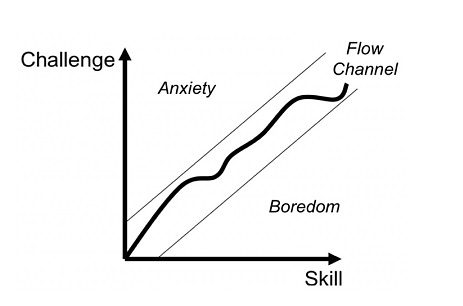
\includegraphics[width=0.6\textwidth]{flowZone}
    \caption{Based on the original model of the flow state)}
    \label{fig:flowZone}
\end{figure}
Over the years, new theories regarding the state of flow have been introduce and the concept flow was redefined by introducing eight experimental channels rather than previously mentioned quadrants \cite{nakamura2014concept}. Figure \ref{fig:flowModel} shows the refined challenge/skill space which now contains a series of concentric rings, associated with increasing intensity of experience.
\begin{figure}[h]
    \centering
    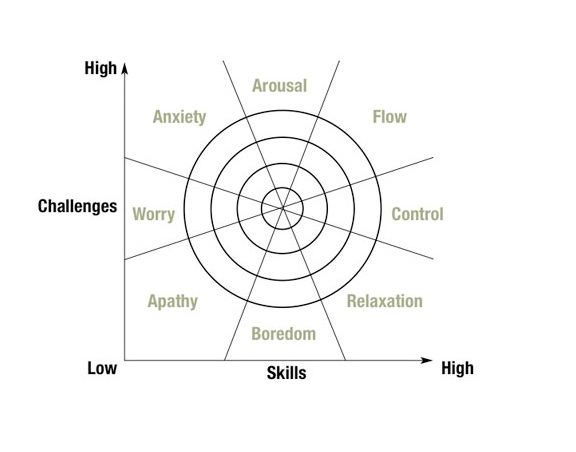
\includegraphics[width=0.6\textwidth]{flow-model}
    \caption{The current model of the flow state \cite{nakamura2014concept}}
    \label{fig:flowModel}
\end{figure}
Based on the current model of the flow state \ref{fig:flowModel}, the flow is experienced in situation when challenges and
skills are above the individual's average levels. When the task is slightly too easy (or slightly too hard) we fall out of the state of flow and enter a state where we feel in control (or the state where we feel aroused if the task is slightly too hard). When the difficulty of the task performed way above our skills, we are tend to experience anxiety. On the other hand, if challenges do not come close to our ability, we will tend to experience boredom. In cases they are below, apathy is experienced. The new model also deals with the intensity of the experience and states the it increases with distance from the individual's average levels of challenge and skill, as shown by the concentric rings \cite{nakamura2014concept}.
Cs\'{i}kszentmih\'{a}lyi \textit{et al.} (2004) also argue how sports and games are more likely to lead to a flow state since they usually have clear goals and feedback structures. However, a given individual can find flow in almost every activity that for some other individuals might seem boring or tiresome \cite{csikszentmihalyi2014flow}.
\subsubsection{Flow in Gamification}
In the context related to human behavior and computers, the concept of flow has been mostly studied in video games, human-computer interaction, instant messaging, to name a few \cite{hamari2014measuring}. Currently, there exist only few studies investigating flow in the context of Gamification (see \cite{hamari2014measuring, sillaots2014achieving}). Thus, and there is insufficient data to draw conclusions as to which of the nine dimensions of flow would be especially emergent in the context of flow. To this end, Hamari and Koivisto (2014) conducted a study in which they investigated the influence and importance of the different dimensions of flow in Gamification.  The data for this study was gathered from users of an exercise gamification service (N = 200) and as a measurement instrument for flow, the Dispositional Flow Scale - 2 (DFS-2) model was used. Introduced by Jackson and Eklund (2002), DFS-2 is designed to access flow experiences in physical activity (see \cite{jackson2002assessing}). The results showed that autotelic experience, clear goals, (immediate) feedback, control and challenge-skill balance were the most salient dimensions of flow in Gamification (of exercise). On the other hand, time transformation, merging action-awareness, loss of self-consciousness were the least salient as shown in Figure \ref{fig:dfs2}.
\begin{figure}[h]
    \centering
    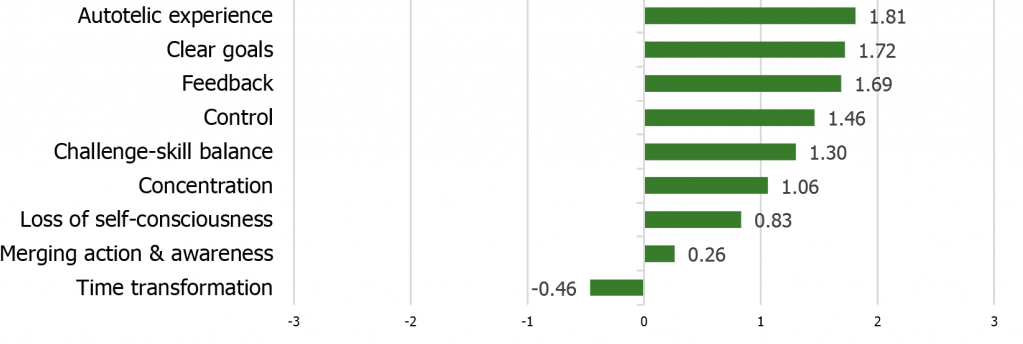
\includegraphics[width=\textwidth]{dfs2}
    \caption{Measuring flow in Gamification: Dispositional Flow Scale-2. Source:  \cite{dfs2}}
    \label{fig:dfs2}
\end{figure}
Furthermore, results also suggest that in gamifed context, the autotelic experience is highly correlated with the conditions. Hamari and Koivisto suggest that it is possible that in the Gamification context, autotelic experience truly represents a condition for reaching flow, thus implying that one can more easily reach flow if the activity is initially intrinsically motivating. 
\subsection{Motivation and Sports}
%pelletier1995toward
Vallerand (2004) states that motivation in sports matters, as it ``represents one of the most important variables in sport''. It is known to be a key element of success in sport and athletes' persistence with an exercise regiment \cite{vallerand2007intrinsic}. Intrinsic and extrinsic motivation have been particularly popular topics that allowed researchers to explain various phenomena of importance in sport and physical activity. Various studies in the domains of health, physical education, exercise and sport have explored the SDT derived hypothesis that intrinsically relative to extrinsically motivated behavior  
TODO: in which areas gamification in sports works already? are there theory parts results that are applicable to our work?...\\*\\*
Armed with a clear understanding of the theory behind human motivation, the following section begins by defining the term Gamification. The goal of this section is to provide an overview of the most relevant key elements of Gamification relevant for the development of iMMotion, in particular why certain game mechanics were the best choice for the iMMotion project.
%In recent years gamifi cation systems were applied in marketing(Muntean, 2011 ; Shneiderman, 2004 ) as well as non-business contexts such as politics,health (Lee & Hammer, 2011 ), or interactive systems (Flatla, Gutwin, Nacke, Bateman,& Mandryk, 2011 ) and education (Lee & Hammer, 2011 ; Raban & Geifman, 2009 ;Rafaeli, Raban, Ravid, & Noy, 2003 ; Ravid & Rafaeli, 2000 ). This rapid developmenthas caught the interest of researchers as a potential to create engaging workplaces(Reeves & Read, 2009 ); facilitate mass-collaboration (McGonigal , 2011 ) or encourageknowledge contribution (Krause & Smeddinck, 2011 ; Shneiderman, 2004 ; von Ahn &Dabbish, 2008 ).
\subsection{Defining Gamification}
As  the  term  itself  is  relatively  new,  there  exist  numerous definitions  of  Gamification  (Zicherman \&  Cunningham 2011, Kapp 2011, Werbach \& Hunter 2012). Definition by Deterding \textit{et al.} (2011) is currently the most cited definition of Gamification in academia and is the definition that is adopted for this thesis. In their paper the authors proposed a well reasoned definition as follows:
\begin{quotation}
\textit{``Gamification is the use of game design elements in a non-game context.''}
\end{quotation}
There exist references to \textit{gamifying} online systems as early as 1980. Professor Richard Bartle from University of Essex, points out the word referred originally to ``turning something not a game into a game.''\cite{werbach2012win}%ovo je knjiga, daj stranu 
However, the first use of gamification in its current sense dates back to 2002 by Nick Pelling as part of his consultancy business, but the term did not see widespread adoption before the second half of 2010 \cite{marczewski2013gamification}. In parallel with this term, a verb \textit{to gamify} emerged. Its meaning refers to applying game mechanics to supercharge user engagement, loyalty and fun \cite{toGamify}. 
It should be noted that the definition outlined by Deterding \textit{et al.} relates to \textit{games} and not \textit{play} \cite{deterding2011game}. %Consequently, the definition distinguieshes between \textit{gamefullness} and \textit{playfullness} ... TODO. 
Even though often used interchangeably, there exists a complex relationship between these two concepts and clear distinction can be made. That is, according to the forms they take in the world, \textit{play} can be interpreted as a broader category that includes \textit{game} as a subset \cite{salen2004rules}. Play is normally assumed to be a free-form activity lacking constraints engaged in for pleasure and amusement rather than a serious or practical purpose, whereas games provide context for actions and are limited in action by fixed rules \cite{juul2011half}. In addition, Salen \& Zimmerman (2004) define game as a system where players engage in an artificial conflict which is defined by rules that limit player's behavior and define the game, that can result in a quantifiable outcome or goal \cite{salen2004rules}. %behavioral, game-playing
Games manifest themselves as integrated experiences, but they are built from many smaller pieces often called game elements \cite{werbach2012win}. They represent parts of games used as a building blocks for creating gamified applications, as well as tools and rules that define the overall context of game \cite{gamDesElem}. This means that the definition distinguishes Gamification from other systems that employ full-fledged games rather than elements of game design only. Furthermore, it does not include all game elements either, only a subcategory called game design elements that are used as seen the most suitable in current situation. %ova dve poslednje recenice odavde, izmeni 
%http://ludus.hu/en/gamification/
The final aspect of the definition is that gamification operates in non-game contexts. A non-game context refers to applications which main purpose is beyond pure entertainment; using game design elements to a context of ``other than games''. This implies that gamification can be used and successfully applied to almost anything: from business, finance, personal improvement to education, health and fitness \cite{deterding2011game}. Thus, the challenge of Gamification, is to select elements that normally operate within the game universe and apply them effectively in the real world.
\begin{figure}[h]
    \centering
    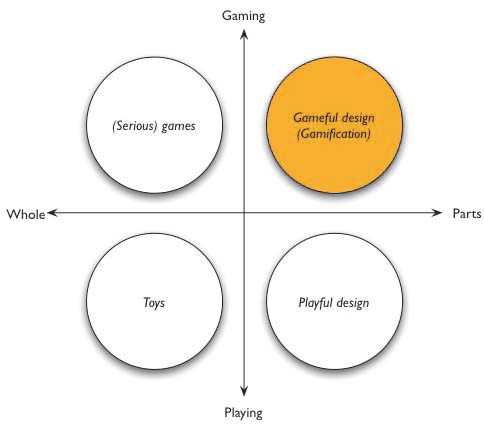
\includegraphics[width=0.75\textwidth]{gamification-btw-game-and-play}
    \caption{The matrix distinguishing the concepts related to gamification}
    \label{fig:mesh1}
\end{figure}
The concept of gamification is closely related to similar pre-existing concepts such as serious games, playful design and toys. Thus, the proposed definition aims at separating the concept of gamification from similar phenomena on a two-by-two matrix introduced by Deterding \textit{et al} (2011, Figure \ref{fig:mesh1}). 
In figure \ref{fig:mesh1}, along one axis a distinction between gaming and playing is made, and on the other between whole game and an artifact with game elements. Gameful design or gamification, differs from playful design because the former focuses on activities that are goal oriented and structured by rules, while the latter focuses on activities that are based on improvisation and are free of form. Moreover, gamification is situated in the quadrant involving games and game elements, meaning that gamification makes use of gameful design rather than playful design and game elements rather than full-fledged games. This is different to serious games used also in non-game contexts, a group that includes full games that have been created for reasons other than pure entertainment. 
\subsection{Defining Exergames}
According to Matallaoui \textit{et al.} (2017), ``one of the most prominent fields where
gamification and other gameful approaches have been
implemented is the health and exercise field'' \cite{matallaoui2017effective}. Even though known for decades, due to the technological advancements which allow more widespread and affordable usage of motion based controllers, these gameful systems and approaches that involve physical activity as the means of interacting with the game, commonly known as \textit{exergames}, have only been proliferating 
in recent years \cite{matallaoui2017effective}. 
According to XXX, the main reason for increased interests in exergames is the concern over high levels of obesity in Western society. Apart from high calorie diet, physical inactivity is considered to be the main reason for obesity, especially among children \cite{kiili2010developing}. Since playing video games is a common leisure time activity among people of all ages, it has been argued by many researchers \cite{kiili2010developing} that video games are one of the main reasons for the decreased level of everyday physical activity and hence, increased level of obesity \cite{vandewater2004linking}. This is what the emerging exergames genre tries to change by encouraging players to perform physical movements during gameplay \cite{kiili2010developing}. Exergames can be defined as ``video games that require physical activity in order to play'' \cite{oh2010defining}. However, a more precise definition of exergame is given by Oh and Yang:
\begin{quotation}
\textit{``An exergame is a video
game that promotes (either via using or requiring) players’ physical movements (exertion) that is
generally more than sedentary and includes strength, balance, and flexibility activities.''} \cite{oh2010defining}.
\end{quotation}
The authors also define exergaming as an: 
\begin{quotation}
\textit{``experiential activity where playing exergames, videogames, or computer-based is used to promote physical activity that is more than sedentary activites and also includes strength, balance,
and flexibility activities''} \cite{oh2010defining}.
\end{quotation}
They main goal is to motivate people to exercise by providing a  ``safe, entertaining and engaging fitness atmosphere'' \cite{altamimi2012survey}.


Researcher at ... showed the exergames can also be used as a fitness tool to help improve and increase the fitness level
The author in [55]
demonstrated this idea using his own body as the main subject
of his experiment. He played three active video games which
differed in the interactions they involved. The three active
games that were used were Dance Dance Revolution which
requires the full body interaction, the EyeToy games which
mainly require upper body interaction and GameBike games
which utilize lower body interaction. After three months of
daily 30 minute sessions plays, two benefits were observed by
the author; weight loss and blood sugar level reduction
\subsection{Player Types}
An important aspect of game thinking is that players differ from one another and their motivation for engaging in gaming activities should not be generalized. That is, people choose to play games for different reasons, and thus, the same video game can have a different meanings or consequences for different players \cite{yee2006motivations}. The more is known about who is playing the game, the easier it is to design and implement an experience that will drive players' behavior in the desired way \cite{zichermann2011gamification}. The  remainder  of  this section will further explore premises about player behavior and personality types. 

\paragraph{Bartle's Four Player Types}

One way to understand players' motivation is to leverage the work accomplished by Richard Bartle in examining player types. Bartle conducted researches in the area of game design and game development and analyzed the ethnography of online game players in the first MUD in 1978 (Multi-User Dungeon). In order to understand why people play games, he identified four main player personality types of MUDs according to specific psychological aspects of their personality and how they prefer playing in a virtual world: \textit{Explorers}, \textit{Socializers}, \textit{Killers}, and \textit{Achievers} \cite{bartle1996hearts}. The player personality types (see Figure \ref{fig:userTypes}) can be defined as follows:
\begin{itemize}
\item \textbf{Explorers} represent players which are driven by motivation to ``find out as much as they can about the 
virtual  world'' \cite{bartle1996hearts}. Not only they enjoy exploring every corner of the game environment and searching for interesting features (i.e. bugs), but also understanding  how 
everything functions \cite{bartle1996hearts}. 
In a sense, for this type of players ``the experience
is the objective'' \cite{zichermann2011gamification}.
\item \textbf{Socializers} are player who play games for the benefit of a social interaction \cite{zichermann2011gamification}. They usually enjoy using communication tools that are provided by the game in order to engage in conversation with other players. 
\item \textbf{Achievers} are goal (achievement) oriented players. They are players who are proud of their ``formal status in the game's built-in level hierarchy'' and also ``of how short a time they took to reach it'' \cite{bartle1996hearts}. This type of players are competitive who enjoy beating difficult challenges whether they are explicitly  set by the game (e.g.  levelling  up  or  gathering  points) or by themselves (e.g. accumulating as much money possible). 
\item \textbf{Killers}, also known as \textit{griefers} \cite{zichermann2011gamification}, are the smallest population of all the player types. They are very similar to achievers, in their motivation for winning, however, these players obtain  enjoyment from causing anxiety and "imposing  themselves  on  others" \cite{bartle1996hearts}. For them, winning is only meaningful if someone else loses.
\end{itemize}
\begin{figure}[h]
    \centering
    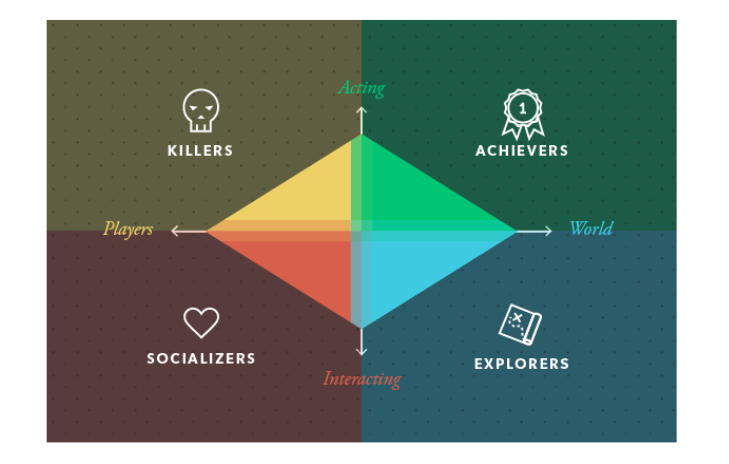
\includegraphics[width=0.75\textwidth]{userTypes}
    \caption{Bartle's Taxonomy of Player Types. Source \cite{bartle}}
    \label{fig:userTypes}
\end{figure}
In the above figure, axes represent the source of players' interest in a MUD. The horizontal axis depicts a preference for interacting with other players vs. interacting with the world and the vertical axis represents a preference for (inter)acting with something vs. (inter)acting on something. Thus, according to the figure, achievers prefer to act on the world, while socializers prefer to interact with other players \cite{bartle}. \\*
It is important to point out that people are not exclusively one or another of the presented player types \cite{zichermann2011gamification}. In their book, Zichermann and Hunter argue that most people have some percentage of each type and the most dominant type will probably change throughout the individual's life. Even though Bartle's player types have not been designed in particular for Gamification it can  help in understanding what attitudes may be dealt with when implementing a gamified solution. 

\paragraph{Marczewski's User Types Hexed}

Bartle's taxonomy of user types was created
specifically for MUDs and it should not be generalized
to other game genres nor to gameful design \cite{tondello2016gamification}. Moreover, it does not consider players who are extrinsically motivated. In order to address these issues Marczewski proposed six user types that differ in the degree to which they can be motivated by either intrinsic or extrinsic  motivational factors \cite{tondello2016gamification} and introduced the \textit{Gamification User Types Hexad framework}.
\begin{figure}[h]
    \centering
    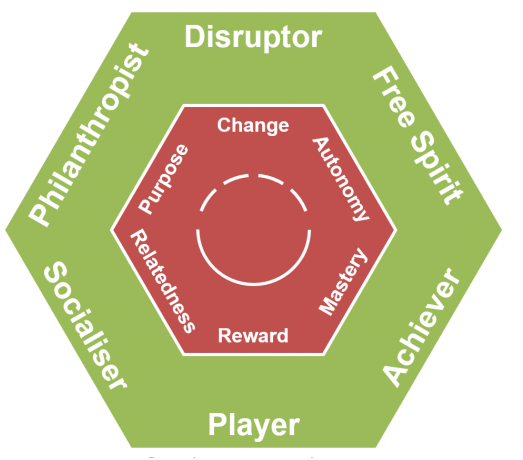
\includegraphics[width=0.75\textwidth]{playerHex}
    \caption{Gamification User Types Hexad. Source: \cite{tondello2016gamification}}
    \label{fig:playerHex}
\end{figure}
\textit{The Hexad} illustrated in Figure \ref{fig:playerHex} is developed in order to identify the users of the gamified system more efficiently, based on users' intrinsic and extrinsic motivations, as defined by SDT \cite{tondello2016gamification}. Marczewski identifies the following types:
\begin{itemize}
\item \textbf{Socialisers} are individuals motivated by \textit{Relatedness}, want to interact with others and create social connections \cite{tondello2016gamification}.
\item \textbf{Free Spirits} are individuals  motivated by \textit{Autonomy} and self-expression. They enjoy the freedom of expression and acting without any external control \cite{tondello2016gamification}.   
\item \textbf{Achievers} are individuals  motivated by \textit{Competence}. As in Bartle's taxonomy, this group seek progress withing the gamified environment by completing various tasks and enjoy proving themselves by overcoming difficult challenges \cite{tondello2016gamification}.
\item \textbf{Philanthropists} are individuals motivated by \textit{Purpose} and \textit{Meaning}. These individuals enjoy giving to others with no expectation of reward in return \cite{tondello2016gamification}.
\item \textbf{Players} are motivated by \textit{Extrinsic rewards}. Motivated only by the reward offered by the gamified system, they will do anything necessary to obtain it, independently of the type of the activity \cite{tondello2016gamification}.
\item \textbf{Disruptors} are motivated by \textit{Change}. In general, they tend to disrupt the system, either directly or through other users to force positive or negative change \cite{tondello2016gamification}.
\end{itemize}
As already mentioned, most people demonstrate each player type to a certain degree. Understanding these player types will support 
the process of choosing the game elements that will be most appealing for the target audience and drive the 
desired behavior. Furthermore, adding features and content in order to appeal to different player types can be of great help to diversify the audience of the gamified system, and create enjoyable experiences for many players.

\subsection{Gamificaton elements}
% \cite{schobel2016agony}.% Sch{\"o}bel \textit{et al.} carried out a literature review to analyze the gamification elements used in various research studies.
%prezentacija o game vs play http://gamification-research.org/2012/04/defining-gamification/
%detering definise elements of game design. five leveles.Next the most common
%Next, and overview and various classification frameworks of game elements which might further enhance engagement, the potential goal of gamification is presented. 
%In a few words, the gamification process can be described as the adoption of some techniques inherited from game design into different situa-tions, other than games. In this perspective, the application of the typical game elements and the exploitation of common game design patterns are used to the aim of making some activities more appealing. In this way, users are stimulated to complete tasks by the desire of getting some rewards (Werbach & Hunter, 2012). Hence, gamification is not related to solve difficult puzzles or avoid tricks but it is the finding of effective ways to drive individuals to their goals faster. Through gamification, people feel involved in the process and are called to be proactive so that they can empower their own abilities and enhance their attitudes both online, in virtual worlds, and offline, in real world situations. Currently, gamification is used by industries to enhance the outcome of their communication campaigns and to drive the attention of people to advertising and marketing messages, in order to maximize their outcome.To conclude, gamification requires a deep understanding of what we can learn from games, so that we can design enjoyable environments and raise passion for the game we are playing  Applying gamification techniques to enhance the effectiveness of video-lessons. Available from: https://www.researchgate.net/publication/283469412_Applying_gamification_techniques_to_enhance_the_effectiveness_of_video-lessons [accessed Mar 5, 2017].
In their book \textit{Gamification by design}, Zimmerman and Cunningham (2011) argue that one should leverage aspects of game design, by focusing on it's core elements, when creating a gamified experience in order to achieve the
greatest impact for players. However, the goal of Gamification is not to build a ``full-fledged game'' but to use game elements in order to provide a gamified experience and enrich the application to engage and motivate the users \cite{werbach2012win, deterding2011game}. With respect to the use of game elements, Gamification studies classified them differently and there have been different attempts to create lists of those game  elements,  which  can  be applied in Gamification \cite{werbach2012win, deterding2011game, kapp2012gamification, zichermann2011gamification}. Derived from the available literature, Deterding \textit{et al.} found that game elements previously identified and presented in different research studies, fell in five distinct levels of abstraction. Table \ref{table:gameElements} presents a model for classification of game elements with five levels of abstraction, ordered from concrete to abstract. Kapp (2012), on the other hand, lists  typical  game  elements  like  goals, time, rules  conflict,  competition,  cooperation, reward  structures,  feedback,  levels,  storytelling,  curve  of  interest  and  aesthetics \cite{kapp2012gamification}. Andrzej Marczewski identified 50 (as of March 2017) elements that support various User Types and can all enhance gamification designs \cite{50GamElements}.
\begin{table}[!htbp]
\centering
\caption{Taxonomy of game design elements by level of abstraction by Deterding \textit{et al.} (2011)}
\label{table:gameElements}
\begin{tabular}{lll}
\hline
\textbf{Level} & \textbf{Description} & \textbf{Example} \\ \hline
\begin{tabular}[c]{@{}l@{}}Game interface\\ design patterns\end{tabular} & \begin{tabular}[c]{@{}l@{}}Common, successful interaction\\  design components and design \\ solutions for a known problem\\  in a context, including prototypical\\  implementations\end{tabular} & \begin{tabular}[c]{@{}l@{}}Badge, leaderboard, \\ level\end{tabular} \\ \hline
\begin{tabular}[c]{@{}l@{}}Game design\\ patterns and\\ mechanics\end{tabular} & \begin{tabular}[c]{@{}l@{}}Commonly reoccurring parts of \\ the design of a game that\\  concern gameplay\end{tabular} & \begin{tabular}[c]{@{}l@{}}Time constraint, \\ limited resources, turns\end{tabular} \\ \hline
\begin{tabular}[c]{@{}l@{}}Game design\\ principles and\\ heuristics\end{tabular} & \begin{tabular}[c]{@{}l@{}}Evaluative guidelines to approach a\\  design problem or analyze a given\\ design solution\end{tabular} & \begin{tabular}[c]{@{}l@{}}Enduring play,\\ clear goals, \\ variety of game styles\end{tabular} \\ \hline
Game models & \begin{tabular}[c]{@{}l@{}}Conceptual models of the components of\\  games or game experience\end{tabular} & \begin{tabular}[c]{@{}l@{}}
MDA; challenge, \\ fantasy, curiosity;\\ game design atoms; \\ Core Elements of the \\ Gaming Experience \end{tabular} \\ \hline
\begin{tabular}[c]{@{}l@{}}Game design\\ methods\end{tabular} & \begin{tabular}[c]{@{}l@{}}Game design-specific\\  practices and processes\end{tabular} & \begin{tabular}[c]{@{}l@{}}Playtesting,\\ playcentric design, \\ value conscious\\ game design\end{tabular} \\ \hline
\end{tabular}
\end{table}
Zichermann \& Cunningham (2011) take a different approach and base their description of game elements on the MDA framework, which is categorized as a \textit{game model} in the framework proposed by Deterding \textit{et al.} (2011). It is one of the most frequently used frameworks of game design and stands for \textit{Mechanics}, \textit{Dynamics} and \textit{Aesthetics} \cite{hunicke2004mda}. 
Introduced by Robin Hunicke, Mark LeBlanc and Robert Zubek, the MDA framework formalizes games consumption by breaking them into their distinct elements: rules, system and "fun". These elements translate into the following design counterparts which constitute the MDA` framework: Mechanics, Dynamics and Aesthetics \cite{hunicke2004mda}. Mechanics are the functioning components that make up the game. They represent the specific elements of the game and the different behaviors and control mechanism that are given to the player within the game's context. Dynamics, on the other side, represents player’s interactions with the mechanics. They specify how the player reacts to the mechanics of the system, both individually and with other players. Lastly, the aesthetics of the system are the emotional reponses of the users who interact with the game system \cite{zichermann2011gamification}. This framework has been very influential in helping designers and theorists conceptualize different aspects of games and how to create them. In their book \textit{For the Win. How Game thinking can revolutionize your business} Werbach and Hunter (2012) introduce three categories of game elements that are relevant to Gamification, which are: \textit{Dynamics}, \textit{Mechanics}, and \textit{Components}. These terms are similar to the ones used in the MDA framework, although LeBlanc \textit{et al} use these terms in different ways. Werbach and Hunter, organized Gamification elements in decreasing order of abstraction where each mechanic is tied to one or more dynamics, and each component is tied to one or more higher-level elements (see Figure \ref{fig:mdc}).
\begin{figure}[h]
    \centering
    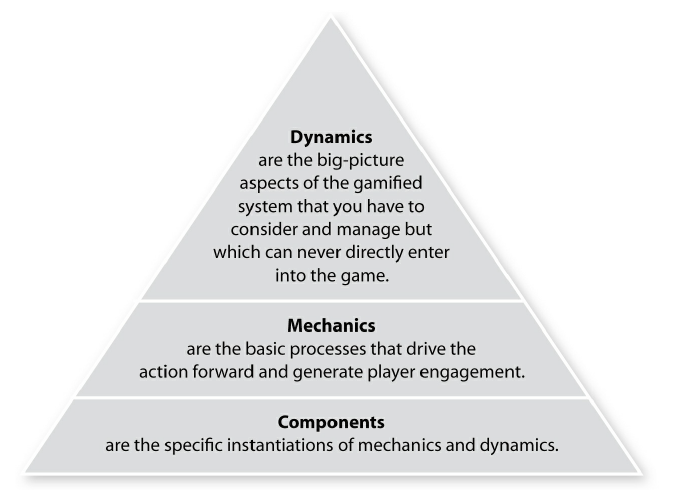
\includegraphics[width=0.75\textwidth]{mdc}
    \caption{The Pyramid of Game Elements from Werbach \& Hunter (2012, p. 82)}
    \label{fig:mdc}
\end{figure}
In the next section different mechanics, dynamics and components are listed and described according to their relevance and applicability to our context.
\subsubsection{Dynamics}
At the highest level of abstraction are game dynamics and serve as the core,  underlying framework for the Gamification to take place. Furthermore, they represent the implicit structure that guide the game, set  up  the  rules and constraints and  define the overall purpose, aim and goal of the game \cite{werbach2012win, WerbachCoursera}. 
According to Werbach and Hunter, the most important game dynamics are \cite{werbach2012win}:
\begin{itemize}
\item \textbf{Constraints}(limitations or forced trade-offs). Every game has some constraints, because games create meaningful choices and interesting problems by limiting people's freedom. So the notion of what constraints get put on users is an important dynamic that any game designer needs to think about. 
\item \textbf{Emotions}. Games can produce various emotions, from joy and sadness to everything in between. However, Werbach argues that the emotional palette of gamification is typically somewhat more limited \cite{WerbachCoursera}. The reason for this is because Gamification deals with real world, non-game context, such as marketing, or exercise context. In contexts like those, getting someone, for instance, really upset, will probable not be beneficial and valued. But there still are a variety of emotional levers that can be pulled, that can make the experience more rich, and certainly the joy, the, the sense of accomplishment, the emotional reinforcement that pushes people to play more, is important in most examples of gamification. 
\item \textbf{Narrative} (a consistent, ongoing storyline) Narrative: the structure that pulls together the pieces of the game, or the gamified system into some coherent feeling whole. The narrative can be explicit, the storyline in a game, or it can be implicit. And gamification doesn't necessarily have the richness of the aesthetic experiential aspect of games to put the work in creating a narrative. It has to rely upon things like consistent graphical experiences, creating a sense of flow and alluding to certain kinds of practices or certain kinds of story ideas that may be in players' heads using those, again, to tie together the individual pieces. If there's no sense of narrative, then the risk is that the gamified system will just be a bunch of abstract stuff. You get these badges. You get these points, but they're totally divorced from any sense of coherence and relation to the player's life and that tends to limit the effectiveness of gamification.
\item \textbf{Progression} (the player's growth and development)
\item \textbf{Relationships} (social interactions generating feelings of camaraderie, status, altruism, and so on)
\end{itemize}
\subsubsection{Mechanics}
Kevin Werbach describes game mechanics as ``the processes that drive actions forward''. He subsequently compared mechanics to ``verbs'' which help people to play games (see Fig. 2). In their academic article, Robert Hunicket et al. defined game mechanics as “the particular components of the game, at the level of data representation and algorithms”.

Mechanics are the basic processes that drive the action forward and generate player engagement. We
can identify ten important game mechanics:

\begin{itemize}
\item Challenges (puzzles or other tasks that require effort to solve)
\item Chance (elements of randomness)
\item Competition (one player or group wins, and the other loses . . . )
\item Cooperation (players must work together to achieve a shared goal)
\item Feedback (information about how the player is doing)
\item Resource Acquisition (obtaining useful or collectible items)
\item Rewards (benefits for some action or achievement)
\item Transactions (trading between players, directly or through intermediaries)
\item Turns (sequential participation by alternating players)
\item Win States (objectives that makes one player or group the winner—draw and loss states are
related concepts)
\end{itemize}
\subsubsection{Components}
Components make up the largest fraction of game elements. They can be viewed as more-specific forms that mechanics or dynamics can take. These elements are less abstract than the categories described previously and lead to tools that can be used in order to begin incorporating Gamification in the environment of interest. There many game elements that can be successfully used in gamified environments. However, some are more common than others, and some are more influential in shaping typical examples of gamification. Werbach and Hunter examined over 100 implementations of Gamification and claim that three elements always appear: \textit{points, badges}, and \textit{leaderboards}. They further point out how these elements are so common within Gamification that ``they are often described as though they are Gamification'', even though they are not \cite{werbach2012win}.  Hamari \textit{et al.} (2014), in their comprehensive survey of peer-reviewed empirical studies on gamification, also found that these three elements ``were clearly the most commonly found variants" in the large variety of elements tested \cite{hamari2014does}. The same elements were listed and described by Zichermann (2011), alongside \textit{levels}, \textit{challenges/quests}, \textit{onboarding}, and \textit{engagement loops} \cite{zichermann2011gamification}. In the next section, these three elements, commonly represented by the acronym \textit{PBL}, will be discussed.
\begin{enumerate}
\item \textbf{Points}\\*
Points represent a running numerical value which is given for any single action or combination of actions. In Gamification, they are mostly used to encourage people to do things by collecting them. The main assumption is that players will work harder in exchange for points. This is a very simple approach that occasionally works in motivating those payer types who like collecting things or who like competing against each other. According to Zichermann and Cunningham (2011) points are ``an absolute requirement for all gamified systems'' and can serve a wide range of purposes, from obvious to barely visible ones. One of the most obvious usage of points and points systems is to for keeping a score. This way, points also provide a way of determining how well someone is doing in the game. So points can either show the relative position of players or they can actually define winning \cite{WerbachCoursera}. Werbach argues that points can also create a connection between progression in the game and extrinsic rewards since gamified systems offer some real-world prizes for reaching certain levels or number or virtual points. Another purpose for points is to provide feedback of the action. Explicit and frequent feedback represent a key element in most good game design, and points provide feedback quickly and easily and, by doing so, they show, in real time, how one is doing in the game. Finally, points provide data for the game designer since the points that users earn can easily be tracked and stored which allows the designer to analyze important metrics about the system. Zichermann and Cunningham (2011) distinguish five categories of point systems. According to the authors, points  can  be  divided  into  different categories  according  to  their  function. That is, one can differentiate among the following point systems: 
\begin{itemize}
\item Experience points,
\item Redeemable points,
\item Reputation points, 
\item Skill points, and
\item Karma  points
\end{itemize}
Each of the mentioned type of point system can have significantly different tasks in the gamified context. Even though, they can be a powerful motivator, Werbach and Hunter state that points are, in fact, very limited because of their uniform, abstract, interchangeable nature. That is, a point is only a point and nothing more. This is one of the reasons why badges are often found in conjunction with points systems.
\item \textbf{Badges}\\*
A badge represents a visual representation of some achievement within the gamified process \cite{WerbachCoursera, werbach2012win}. It should be noted that terms badges and achievements are often used interchangeably in
Gamification. They are a visual indication that a player has reached a certain level or accomplished some set of objectives \cite{werbach2012win, zichermann2011gamification}. When acquired, badges can serve a success indicator and, thus, possibly inspire players to achieve more badges. A well designed badge system, according to researchers Judd Antin and Elizabeth Churchill has five motivational characteristics \cite{werbach2012win}:
\begin{enumerate}
\item Badges can provide a goal for users exert oneself toward, which can positively affect players motivation
\item Badges can guidance as to what is possible and achievable within the system 
\item Badges are a signal of what a user cares about and capable of achieving. Thus, they are a visual marker of a player's reputation. That is the reason why players will often strive to acquire badges in order to show
others what they are capable of.
\item Badges can operate as virtual status symbols 
\item Badges can function as tribal markers. To put it more simple, a player who acquired some badges same as other players will feel a sense of identity and belonging with that group
\end{enumerate}
Werbach and Hunter point out that one of the most important attributes of badges is their \textit{flexibility}. That is, the possibilities with badge systems are immense and limited only by the imagination of the Gamification designer and the needs of the business. This allows the gamified system to target and suit the interest of a more diverse group of users in a way that is unachievable for a single point system \cite{werbach2012win}. 
\item \textbf{Leaderboards}\\*
The main purpose of a leaderboard is to make simple comparisons among players and to give context to progression in a way the points or badges usually can not. \cite{zichermann2011gamification, werbach2012win}. According to Werbach, in a context where performance matters, leaderboards can be very powerful motivators. That is, if a player sees that only few points are needed for moving up a slot or to emerge on top, it can be a strong motivator for pushing oneself harder in order to achieve that goal. However, in some situations leaderboard can be demotivating. In cases when the ranking lacks meaning or one notices how far behind the top ranked players is, a player can even decide to leave the gamified environment. According to Zichermann, there are various types of leaderboards used in gamified systems nowadays. However, the author encourages the usage of the \textit{no-disincentive leaderboard} in which, independent of the ranking order, the player is placed in the middle of the leaderboard where only the player's with a similar score can be seen. That way, one only sees how much is needed for the next best score, thus the possible demoivation by seeing how much is one behuind the top scored players is most probably avoided. A variant of this type of leaderboard, also used often in gamified systems, is the \textit{friend relative leaderbord} that only shows the score of people who are in the player's social graph. In this case, the player's score is compared not just to stranger but to people one is friends with \cite{WerbachCoursera}. Werbach, furthermore, points out that leaderboards do not need to track only one attribute, but it is up to the designer of to decide which attributes to be tracked. 
\end{enumerate}
The \textit{PBL triad} represents a useful starting point for building gamified solution, however, relying only on them can lead to negative outcomes \cite{werbach2012win}. This is because elements do not make the game \cite{werbach2012win, WerbachCoursera}. They are great tools for communicating progress and acknowledging effort, but neither points nor badges in any way constitute a game. This is where problems emanate. Heavily relying only on these elements, without understanding other aspects of game design could suppress players' intrinsic motivation, that is, their desire to engage with a game (or gamified service). However, no actual empirical evidence exists to back this claim \cite{mekler2013points}. Furthermore, when using the PBL triad, the most emphasis is put on rewards. The problem with this, according to Werbach, is that ``not all rewards are fun; not all fun is rewarding'' \cite{WerbachCoursera}. Thus, heavily relying only on rewards, might demotivate players in further engagement with the gamified system. On the other hand, Werbach claims that what can make elements successful is the ``way they are all tied together'', which often involves some higher level concepts such as dynamics. To sum up, even though PBLs have huge potential, they are not right for every project. That is why, some other elements should also be considered in order to ``extract the maximum value from Gamification''\cite{werbach2012win}. \\*
Apart from the described ones, there are other gamification mechanics that can be used, and these were identified by Werbach and Zichermann in their respective books. To 
In most games and gamified systems, levels indicate the players progress or they can serve as a marker reflecting the achievements and competence of the player in a gaming experience over time \cite{zichermann2011gamification}. Some of the most common are \cite{zichermann2011gamification, werbach2012win} 
\begin{itemize}
\item Achievements (defined objectives)
\item Avatars (visual representations of a player's character)
\item Collections (sets of items or badges to accumulate)
\item Combat (a defined battle, typically short-lived)
\item Content Unlocking (aspects available only when players reach objectives)
\item Gifting (opportunities to share resources with others)
\item Levels (defined steps in player progression)
\item Quests (predefined challenges with objectives and rewards)
\item Social Graphs (representation of players' social network within the game)
\item Teams (defined groups of players working together for a common goal)
\item Virtual Goods (game assets with perceived or real-money value)
\end{itemize}
According to Werbach the central task of a gamification design is putting all these elements together. However, one should keep in mind that no gamification system will and need to include all of these elements. On the other hand, it is necessary to take into account all the possible elements in order to build an engaging gamified service \cite{werbach2012win}. 

%just for health and fitness gamification
%First  the  elements  most related   to   motivation   are   presented   and   then   the   most   popular elements   in gamification  literature  are  presented.  Although  all  game  elements  can be  used  in gamification they might not all be equally relevant. Some are more potent and useful than others. As it is also a goal of this paper to examine which elements are the most  relevant,  based  on  the  research  done  on  motivational  theory  and  gamification literature a distinction is made.
%In theory, any context, task or process can be gamified \cite{muntean2011raising}. %skini i procitaj Muntean!! 

%\subsection{Objectives}
%\subsection{Principles}
%\subsection{The impact of Gamification}
%\subsubsection{Gamification in sports - Effects and Objectives}
%The main goal of gamification is to engage the users Gamification’s main goal is to rise the engagement of users by using game-like techniques such asscoreboards and personalized fast feedback (Flatla et al, 2011) making people feel more ownership and purpose when engaging with tasks (Pavlus, 2010).\cite{burke2016gamify}
%\subsection{Gamification critiques}

\subsubsection{Elements and Player Types}

\subsubsection{Gamification Design}

\subsection{Gamification of Health and Fitness}
Gamification in Health and Fitness has rapidly emerged over the past decade as a tool to promote health and wellness, as evidenced by the number of applications found in Apple App Store and Google Play Store containing at least some Gamification element. 

 %The best examples of gamification are in the Health and Fitness industry, where games encourage exercise by turning physical activity into a game and by delivering health interventions for bad habits cessation, like smoking, overeating or poor hydration, and medication adherence. Application of mobile and wearable devices have proven to be effective platforms for health and fitness games due to its wide adaptation, ease of use and continuous proximity to the users and patients. Since gamification can be applied to almost any business model, serious or not, for this thesis, we restrict our concern of gamification to the solving of serious issues. In particular, we are focused on gamification of education and behavior change related to the serious world issue of childhood obesity
